\chapter{Introduction \& Motivation}
\label{chapter:introduction}
\begin{music}
    \parindent10mm \instrumentnumber{1} \setstaffs1{1} 
    \generalmeter{\meterfrac34} \generalsignature{3}
    \startextract
            \Notes \Dqbu dk \zhl{i*} \en
        \bar
            \Notes \Dqbu hi \zhu{h*} \en
    \zendextract
\end{music}
\epigraph{\textit{one thing that won't change with time is the memories of younger years}}{Minuet of Forest --- Ocarina of Time}

We are living in the wake of milestones in biotechnology and computational biology that suggest reverse-engineering cell biology is within our grasp. The coronavirus pandemic accelerated investment in biotechnology \cite{DeFrancesco2021Financing2020}. The fields of synthetic and systems biology are beginning to resemble engineering disciplines; genetic engineering is becoming more precise, high-throughput single-cell experiments are performed by robots and measurements across all levels of the central dogma are possible: genomics, transcriptomics, proteomics and metabolomics \cite{Perkel2021Single-cellAge}. Advances in micro-fabrication \cite{Shafiee2017TissueMedicine} and in-vitro reconstitutive methods \cite{Gopfrich2018MasteringCells} have allowed biologists to isolate pathways and mechanisms to a level of mathematical and computational tractability \cite{Sharpe2017ComputerTomorrow.}.

The complexity barrier in biology poses a significant challenge. Multiple levels of organisation from the molecular, to cellular, to the whole organism interact with each other, which makes scale separation and accurate approximations difficult. Furthermore, the combinatorial space of possible interactions between macro-molecules involved in the central dogma is intractably large. Systems and synthetic biology have historically made progress through a process of brute force trial and error. This usually involves the interaction of many custom-made parts that are iteratively optimised by human intervention. A trend first observed in the 1980s known as \textit{Eroom's law} revealed that discoveries in biotechnology are becoming slower and more expensive over time, despite improvements in technology \cite{Scannell2012DiagnosingEfficiency}. This problem is exemplified by the declining success rate of clinical trials in the drug discovery process \cite{Wong2019EstimationParameters} and compounded by the ongoing reproducibility crisis \cite{Ioannidis2005WhyFalse.,Mullard2021HalfEffort}. It appears that much of the low-hanging fruit has been picked \cite{Earm2014IntegrativeDevelopment} with methodologies whose standards for transparency, reproducibility and accessibility leave us with much to be desired. 

Despite the widespread lack of mechanistic understanding in human cell biology, sophisticated engineering goals such as targeted modification of the immune system are now possible. In 2018, a T-cell gene therapy --- \emph{tisagenlecleucel} \cite{Halford2021TisagenlecleucelConsiderations} --- for the treatment of adolescent and young adult acute lymphoblastic leukaemia became the most expensive cancer therapy ever, at \$475,000 \cite{Hernandez2018TotalImmunotherapy}. Here, the high cost results from a hugely complex procedure for administering the treatment, which involves harvesting patient T-cells and engineering them to express a novel chimeric antigen receptor (CAR), and then returning the modified T-cells back into the patient. Even in settings where biomanufacturing relies on specific known mechanisms, the manufacturing of viral vectors that deliver the gene therapy is far from straightforward. Human-derived producer cells are used to  synthesise vector \cite{Merten2016ProductionVectors}, but how to engineer them to carry this out efficiently depends on understanding the complexity of these complex cell-types, which involve a great number of unknown mechanisms. To provide clues into the biological processes that limit efficient bioproduction, omics data can be collected along key protocol stages in attempts to understand and optimise production.

After a decade of engineering advances in data science and machine learning, epitomised by deep learning methods, theoretical foundations on high-dimensional learning tasks are beginning to condense \cite{Bronstein2021GeometricGauges}. Many tasks such as computer vision \cite{mnist2012,imagenet2009}, playing Go, or protein folding \cite{Jumper2021HighlyAlphaFold} are in fact feasible with appropriate computational scale. Remarkably, the essence of deep learning is built from two simple algorithmic principles: the notion of lower-dimensional \emph{representation}, whereby group equivariant and invariant transformations are composed to capture the appropriate notion of regularity for each task \cite{Bronstein2021GeometricGauges}, and second, learning by local gradient-descent type methods enabled by \emph{differentiable programming} \cite{Innes2019AComputing}.

The emerging picture suggests that bringing together the advances in software and wetware in iterative hypothesis generation and discovery pipelines are key to overcoming the complexity barrier in biology \cite{Sharpe2017ComputerTomorrow.,Ringel2020BreakingLaw,AlQuraishi2021DifferentiableMechanisms}. The term \textit{in silico} has become popularised amongst biologists, which conceptualises a computational model, alongside \emph{in vitro} and \emph{in vivo}, as a method for investigating an organism \emph{in situ}. Researchers are going as far as conceptualising the \emph{digital twin} for personalised medicine \cite{Bjornsson2019DigitalMedicine}. Bringing together deep learning and biomedical research has the potential of importing the notions of \emph{representation} and \emph{differentiability} into biological engineering \cite{AlQuraishi2021DifferentiableMechanisms} and thereby reaping their benefits. Differentiability within engineering pipelines has the same advantage over brute force trial and error as it does over sampling-based algorithms and thereby decrease the time and cost for biological research. While not all equipment, data and resources used to perform a study can be shared, representations of a study in the form of computational models can increase transparency and reproducibility. Efforts towards open standards have gained traction over the past decade \cite{Malik-Sheriff2020BioModels15Science} with model sharing standards such as Systems Biology Markup Language \cite{Hucka2018TheCore} and data repositories like Human Cell Atlas
\cite{Regev2017TheAtlas} and Flow Repository \cite{Spidlen2012PreparingFlowRepository.org}. The open standards and ethical thresholds of deep learning are also increasing, with the formation of OpenAI \cite{Brockman2016OpenAIGym} and sharing standards such as ONNX \cite{Bai2019ONNX:Exchange}.

\section{Representation of Single Cells}

In this thesis, the focus is on differential equation representations of single cells. In this section we give a brief motivation behind why differential equations are convenient, what other representations exist and how results may translate between differential equations and other representations. When studying a particular biological phenomenon, the appropriate spatio-temporal scale must be chosen that simplifies the mechanism under study while preserving the relationships between experimentally accessible parameters and the resultant behaviours. We do not expect a single unifying tractable model of biological mechanisms under study. In practice there exist multiple equally valid models with various degrees of complexity. For example, the immune system can be described with agent-based models \cite{} and also with ordinary differential equations \cite{}. The set of equations can describe all molecular interactions within a cell \cite{}, or only the pathways under study \cite{}. In cases where tissue organisation or sub-cellular spatial mechanics are important, partial differential equations \cite{}, vertex models \cite{} and \cite{} can be used to characterise them.
\begin{Figure}
    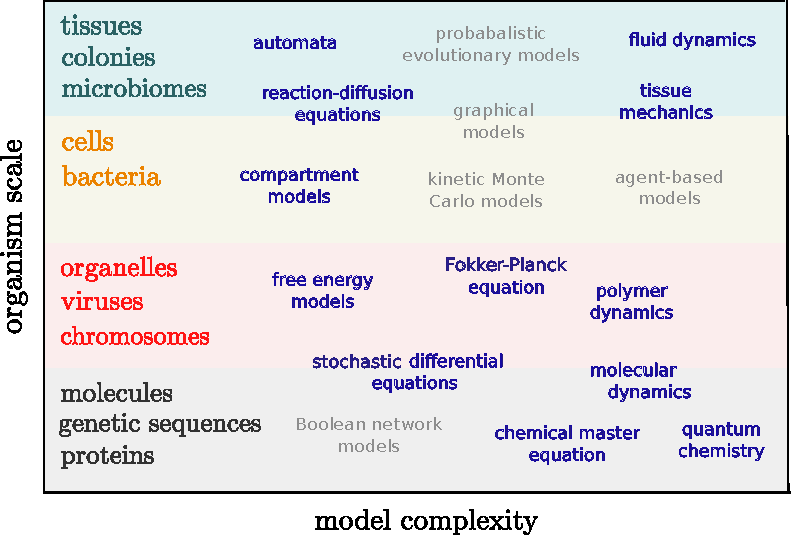
\includegraphics[width=0.9\linewidth]{figures/top-down-bottom-up}
    \caption{Biological models at different spatial scales and complexities, a large class of which can be cast into differential equation form indicated in bold blue}
    \label{fig:tdbu}
\end{Figure}
Differential equations are convenient because they are usually differentiable, continuous state and continuous time models and hence are already compatible with the two algorithmic principles of deep learning \cite{Bronstein2021GeometricGauges}. In the context of dynamical systems theory it is relatively simple to derive analogous results for discrete state or discrete time models: cellular automata \cite{Martin2017DifferentiableAutomata}, Markov chains \cite{Darling2008DifferentialChains}, stochastic processes and discrete maps just to name a few. A large class of biological models at different spatial scales can be cast into differential equation form (Figure \ref{fig:tdbu}), although this may not always be necessary. With the help of automatic differentiation, programs with arbitrary control flow become piecewise differentiable \cite{Gune2018AutomaticSurvey}. One of the main limitations to consider is the number of branches in the program due to conditional statements and whether there are non-zero derivatives either side of the conditional statement that provide meaningful information. Rule-based models such as agent-based models are examples of programs with many conditional branches often with no meaningful derivatives on either side of the condition. In such scenarios we must fall back to finite difference approaches, requiring a finite number of evaluations of the model. This can be done in a cost-effective way, only evaluating gradients that will likely benefit the optimisation.

Differential equations models span a large range of spatial and temporal scales. It is important to choose a time-scale and space-scale that is relevant to the problem. If one is interested in tissue dynamics, attempting to model DNA conformations within each cell will render the problem intractable. As George Booth aptly put \textit{``most models are wrong but some are useful"} so the role of theoretical descriptions in these settings is not necessarily to describe the way reality \textit{is} but serve as tools to bridge the non-intuitive gap between bottom-up and top-down approaches \cite{Gopfrich2018MasteringCells,Powell2018HowScratch,Pezzulo2016Top-downLevel}.

\subsection{Model Selection \& Reduction}
With such a heterogeneous selection of models that are valid at different spatial and temporal scales it becomes increasingly important to develop tools to navigate the space of models. We want to organise and then choose between different models that explain the same phenomenon whilst also enumerating the set of phenomena that a single model can explain. This problem is known in machine learning as model selection \cite{Ding2018ModelOverview} and establishing relationships between models of varying complexity is know as model reduction \cite{Besselink2013AControl}. We will see in the following section that exploring the space of models inherently involves some form of iterative hypothesis generation workflow.

In the context of parameter inference \cite{Brunton2016SparseSINDYc,GorbachScalableSystems}, sloppiness and sensitivity analysis have been extensively used in the search for reduced models \cite{Daniels2008,Chis2016OnIdentifiability,Gutenkunst2007UniversallyModels,Gabor2017ParameterBiosystems,Villaverde2016StructuralModels}. Linear mappings between models that preserve stoichiometry and reactant structure were investigated \cite{Cardelli2014MorphismsFunction,Cardelli2017MaximalSystems} and computational tools based on partition-refinement were released \cite{Cardelli2017ERODE:Equations}. Structural similarity between reaction networks can be revealed by such mappings, elucidating the functional aspects of complex networks in terms of simpler networks. Nonlinear mappings between models that preserve high-level features without resorting to structural assumptions about the models were still lacking lacking and formed part of the motivation for developing the methods in Chapter \ref{chapter:inference}.

We will see how a suitably defined cost function that focuses on high-level features of a model enables navigation and organisation of models across various levels of complexity. Indeed the focus on higher-level features of differential equation models, such as geometry rather than kinetics, has already been gaining traction in 
pattern formation theory \cite{Halatek2018}.

\section{Differentiability in Biological Engineering}

While there is a clear mathematical definition of what a \emph{differentiable program} \cite{Innes2019AComputing} is, what does it mean for engineering in biology to be differentiable? In the effort to move past brute force trial and error methods, a standard for the \emph{design--build--test--learn} cycle has emerged in synthetic biology (Figure \ref{fig:dbtl}). This workflow has now been established as a paradigm \cite{Carbonell2018AnChemicals,Opgenorth2019LessonsLearning} with some aspects that have been automated by liquid handling robots, bioreactor environments and image processing pipelines. However, humans in the loop and custom moving parts still persist. Defining the boundary between parts that can be automated, and parts that need regular intervention by domain experts is a challenge \cite{Abate2018ExperimentalSemantics}.
\begin{Figure}
    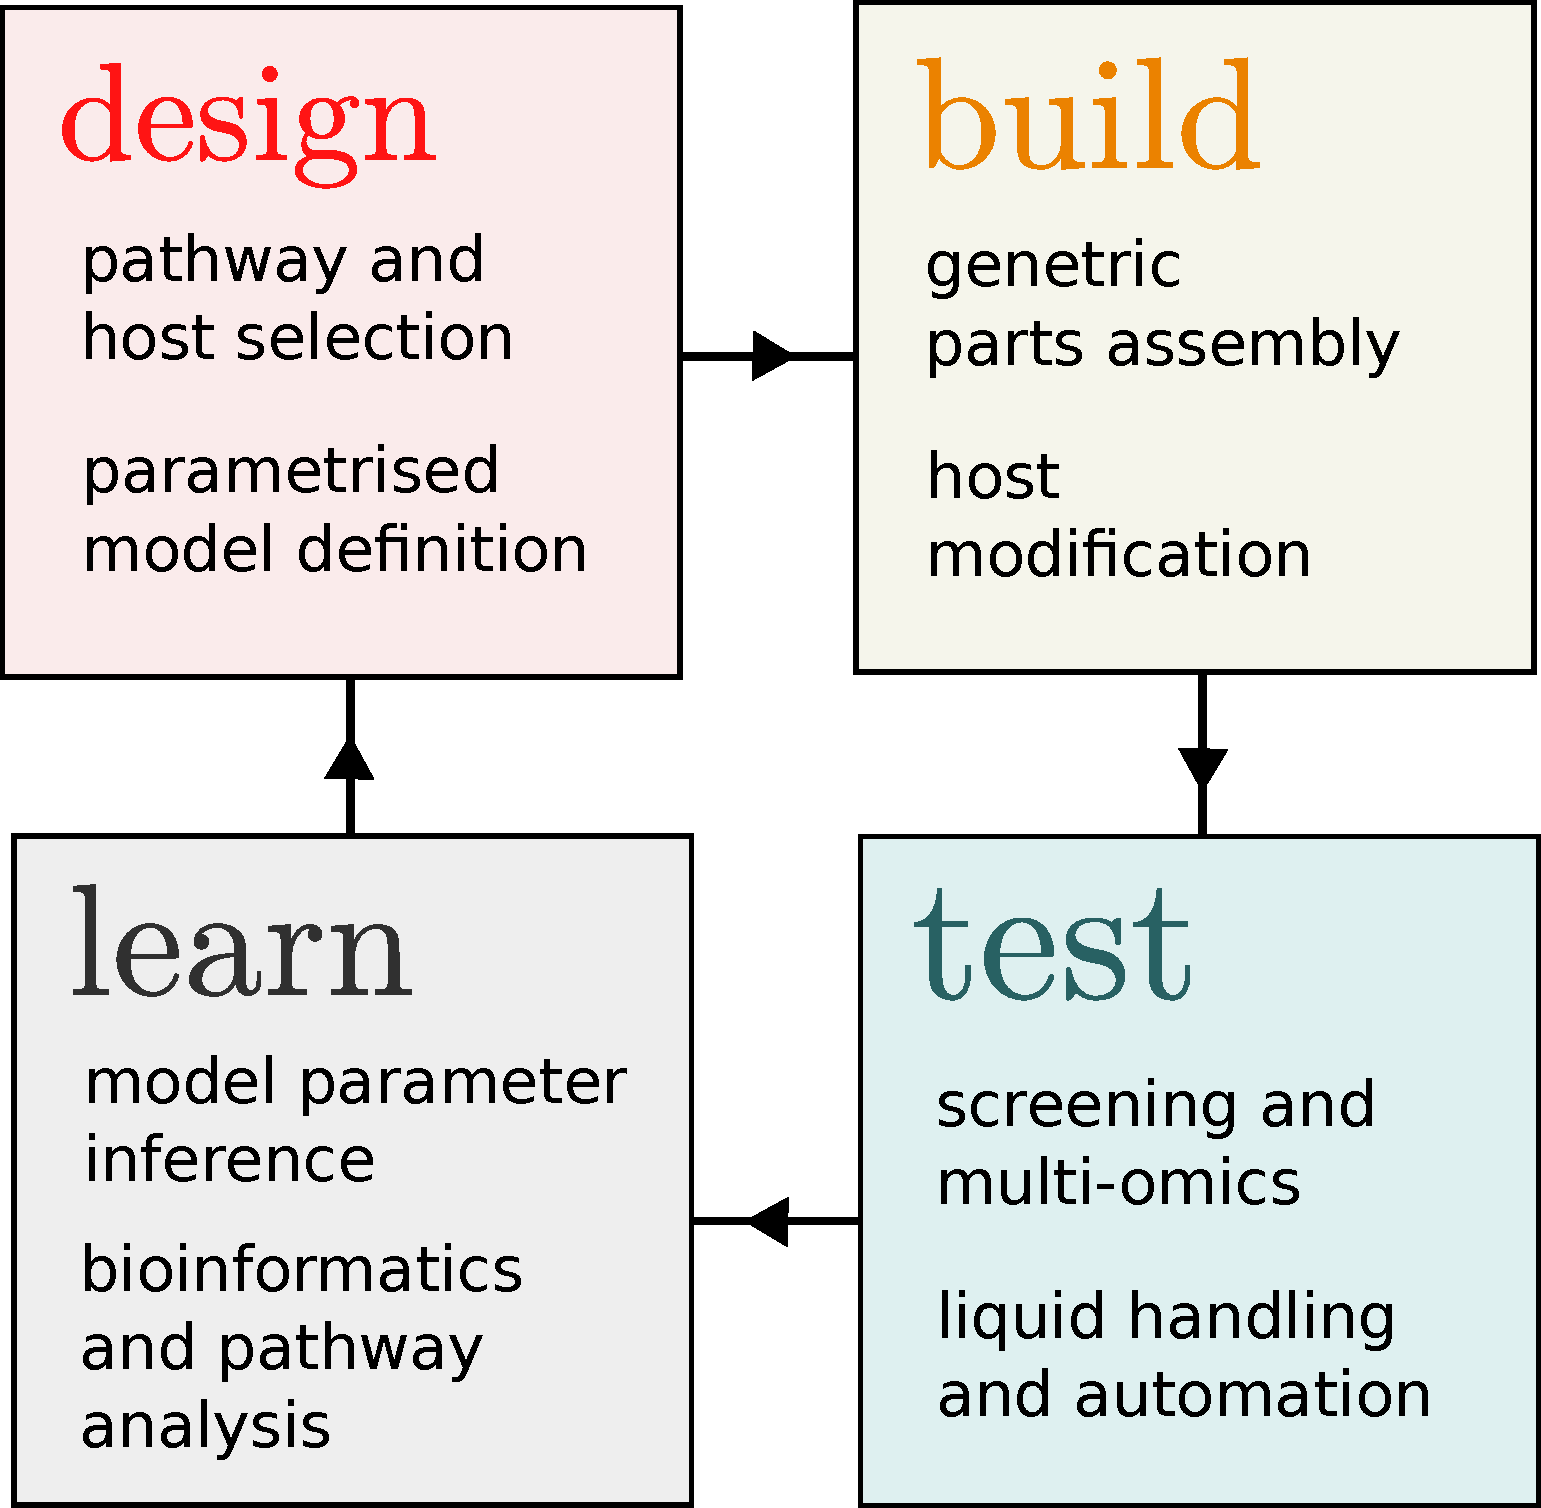
\includegraphics[width=0.6\linewidth]{figures/dbtl}
    \caption{\emph{design--build--test--learn} cycle from synthetic biology. This cycle is differentiable if a domain expert can track changes in any observation pair \emph{X,Y} along the pipeline}
    \label{fig:dbtl}
\end{Figure}
In principle such a pipeline is differentiable if a domain expert can efficiently get an answer questions like: \emph{What happens to Y when I change X?} or \emph{Which X do need to change in order to change Y?} for as many observable pairs \emph{X,Y} as possible. Furthermore, suitable experiments are identified to the capture the relevant data.

The \emph{design--build--test--learn} paradigm was used during the interdisciplinary collaboration described in Chapter \ref{chapter:double-exclusive}. In this thesis we focus on the \emph{design--learn} part of this workflow. One of the main learnings, as we shall see, from applying this paradigm is that, in order for the lab to converge onto their cell design goals efficiently, the workflow must be bidirectional, rather than a cycle. This way each part of the workflow can operate with its neighbours independently, without being blocked by other parts of the workflow.

\subsection{Design--Learn Workflow}
\label{section:design-learn}
Let us focus on the \emph{design--learn} part of the workflow in the context of model inference. Partial knowledge of mechanisms in biology has given rise to a class of models that have been coined as \emph{grey box models} \cite{Meeds2019EfficientSystems}. In this setting, domain expertise dictates which aspects of the model are highly structured with specific hypotheses and which are composed with generic transformations that obey a chosen set of group symmetries.
\begin{Figure}
    \begin{tikzpicture}[node distance=2cm]

        \node (nonparametric) [process, minimum width=5cm] {unstructured inference};
        \node (data) [io, right of=nonparametric, xshift=1cm, yshift=2cm] {observations $\mathcal{D}$};

        \node (field) [decision, below of=nonparametric] {model $F$};
        \node (pred) [io, right of=field,  xshift=2cm] {predictions};

        \draw [arrow] (data) |- (nonparametric);
        \draw [arrow] (nonparametric) -- (field);
        
        \draw [arrow] (field) -- (pred);
        \draw [arrow,color=BurntOrange] (pred) -- +(0,3.5);

    \end{tikzpicture}
    \caption{\emph{Design--learn} workflow without mechanistic knowledge. Predictions generated from the model $F$ are only accurate in the vicinity of data $\targets$}
    \label{fig:experimental-design}
\end{Figure}
Consider time-course gene expression data $\mathcal{D}$, which could be taken via time-lapse microscopy of cells growing on microfluidic plates, optical density measurements from microtiter plate assays or temporal snapshots of flow cytometry measurements. If nothing is known about a mechanism under study, we can infer an unstructured model from a set of observations, and even generate predictions without needing to know anything about the mechanism (Figure \ref{fig:experimental-design}). Unstructured models do not generate accurate predictions outside the input data distribution; they are good interpolators, but terrible extrapolators.

Models $\rates$ constructed with feasible biophysical assumptions have the potential to extrapolate predictions and give concrete biophysical meanings to each parameter $\theta$. This way the experimentalist knows exactly which modification to the system they must make in order to achieve a desired behaviour. More often than not it is also unclear whether the model and its assumptions are reasonable, which brings us to model selection and reduction (Figure \ref{fig:non-parametric}). 
\begin{Figure}
    \begin{tikzpicture}[node distance=2cm]

        \node (field) [decision] {model $F$};
        \node (hypothesis) [io, left of=field,  xshift=-2cm] {hypothesis $\rates$};
        \node (parametric) [process, below of=field, minimum width=5cm] {model selection};
        
        \node (decomp) [process, below of=parametric, minimum width=5cm] {model reduction};
        \node (models) [io, left of=decomp, xshift=-3cm] {models};

        \draw [arrow] (field) -- (parametric);
        \draw [arrow] (hypothesis) |- (parametric);
        \draw [arrow] (parametric) -- (decomp);
        
        \draw [arrow] (decomp) -- (models);
        \draw [arrow,color=ForestGreen] (models) -- +(0,3.5);

    \end{tikzpicture}
    \caption{Overview of model selection, reduction and refinement loop}
    \label{fig:non-parametric}
\end{Figure}
Alternatively one may construct $\rates$ to cover a whole class of models rather than a single model. The expectation is that most of the parameters would be zero but some would be informative \cite{Brunton2016SparseSINDYc}. From the inferred parameters $\theta$ one may construct alternative hypotheses and narrow down the set of plausible models. By iterating this procedure one would identify the minimal model within the model class that explains the data.

\section{Thesis Content Summary}
In this thesis we focus on the benefits of differential equation representations and differentiable \emph{design--learn} workflows in the context of the genetic engineering of cell phenotypes in synthetic biology. In Chapter \ref{chapter:background} we introduce the reader a relevant background in differential equations and machine learning with applications in cell biology to set the stage for the publications in Chapters \ref{chapter:double-exclusive}--\ref{chapter:exploring}. We will see how a differential equation representation of a cell or population of cells requires an exploration of the relationship between bifurcation theory and the concept of a phenotype. Chapter \ref{chapter:double-exclusive} exhibits the results of an interdisciplicary collaboration between in synthetic biology, during which an iterative \emph{design--learn} workflow was followed in an attempt to overcome the biological complexity barrier. During this collaboration, a disconnect between design goals and parameter inference methods was identified which lead to the novel bifurcation inference method published in Chapter \ref{chapter:inference}. Chapter \ref{chapter:exploring} is an adaptation of a publication, in preparation at the time of writing this document, that explores the importance of interactive exploration of high-dimensional flow cytometry data for immunophenotyping. Finally, Chapter \ref{chapter:conclusions} concludes with retrospectives on the previous chapters, which includes a revised view of a \emph{design--learn} workflow for synthetic biology, that in principle is completely differentiable. Furthermore, we propose how one would use concepts from Chapters \ref{chapter:inference}--\ref{chapter:exploring} to interactivity explore the space of hypotheses that represent the same cell phenotype. Our conclusions would be most impactful in cell line development where flow cytometry and other omic-type measurements are taken at different protocol stages of a biomanufacturing process.